
\section{ByteNet}

\subsection{Validating Implementation}

Before using the model on the Europarl v7 dataset for solving the WMT Translation Task problem, the model is validated using some simpler datasets.

\subsubsection{Learning Synthetic Digits Problem}

The Synthetic Digits dataset is used for validating the generalization properties of the ByteNet implementation.

The internal dimensionality is set to 20, this is 20 units in the encoder and 40 units in the decoder, the latter is because the encoding is concatenated with the target embedding. It is unlikely that higher dimensionality is required, given that there are only 10 possible output characters. In fact, 20 might be much higher than necessary, but this may be a good thing in terms of validation as it provides an opportunity to ensure that the model doesn't overfit. Using a dimensionality of 20 the network has, just counting the convolution and dense layers, $73500$ weights. The training dataset contains only 128 observations, thus there is a huge potential for overfitting. The test dataset also contains 128 observations.

The ByteNet model is optimized using the MaxProp optimizer with a learning rate of 0.001 and a mini-batch size of 16 running on 1 GPU. Because the BLEU score is not meaningful for the Synthetic Digits problem, where no words exist in the target, the misclassification rate is calculated instead.

\begin{figure}[h]
    \centering
    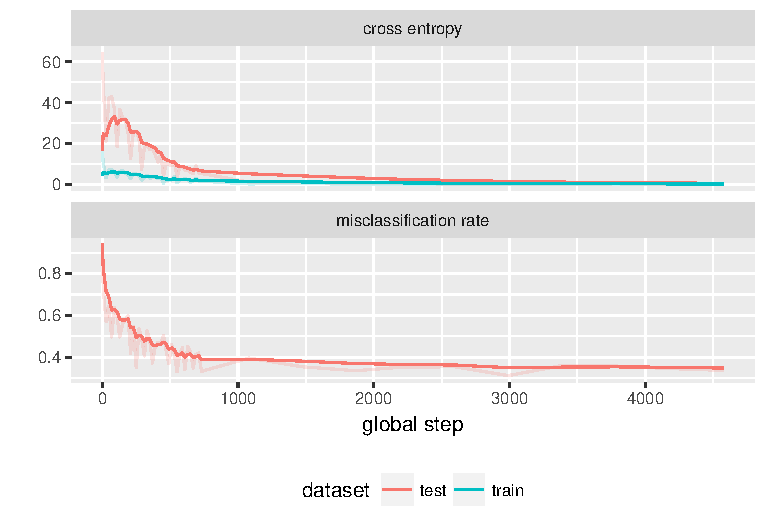
\includegraphics[scale=1]{bytenet/validation-synthetic-digits.pdf}
    \caption{Shows misclassification rate and the cross entropy loss. For comparison a the attention model has misclassification rate at 0.51. The exponential moving average used a forget factor of $0.4$.}
    \label{fig:result:bytenet:digits}
\end{figure}

\begin{table}[h]
\centering
\begin{tabular}{r|p{3.3cm} p{3.3cm} p{3.3cm}}
	obs. & source & target & predict\\ \hline
  0 & one zero four & 104 & 104 \\
  1 & one five six & 156 & 15 \\
  2 & five five nine & 559 & 559 \\
  3 & one six & 16 & 10 \\
  4 & two three four & 234 & 212 \\
  5 & five three & 53 & 53
\end{tabular}
\caption{Source, target, and prediction on examples from the test dataset.}
\label{table:result:bytenet:digits}
\end{table}

Figure \ref{fig:result:bytenet:digits} shows reasonable convergence, only the test error shows jitter during training and there is very little overfitting if any. In the end, the ByteNet model completely learned the training dataset.

The jitter is likely not because of poor optimization, but rather because the errors are only calculated on a randomly sampled subset of the test dataset. For the different samples, the test error is different.

The lack of overfitting fits well with what the original ByteNet article also observed, in their translation model no regularization or early stopping was used, which is what one would typically use to prevent overfitting \cite{bytenet}.

In table \ref{table:result:bytenet:digits} the predictions are about what one would expect. For the most part, the translation, in particular in the beginning of the output sequence, while the latter digit predictions show some error. This result is reasonable, as there is more data for the first two digits and because the input words have different length, the alignment between input and output characters becomes more uncertain. Of cause, the model would ideally learn the word separation completely and understand that there is a direct relation between word and digit, but they are likely difficult given both the many parameters and the small dataset.

\clearpage
\subsubsection{Memorizing WMT NewsTest}

Sometimes a model works well when it has few weights and low dimensionality but breaks for higher dimensionality because of vanishing or exploding gradient issues. To validate that this is not an issue a good test is to see if the model can memorize a small dataset, but where the model complexity is kept high. For memorization one just expects the training loss to become very small, the test error is not important.

The WMT 2014 NewsTest dataset for German to English translation was used for training, this contains 3003 observations. The WMT 2015 NewsTest dataset was used for testing, this contains 1596 observations. The internal dimensionality is set to 400, (800 in the decoder because of concatenation).

The model ran 300 epochs over the training dataset, with a mini batch size of $4 \cdot 16 = 64$, running on 4 GPUs in parallel using synchronized updates with the MaxProp optimizer and a learning rate of 0.0001.

\begin{figure}[h]
    \centering
    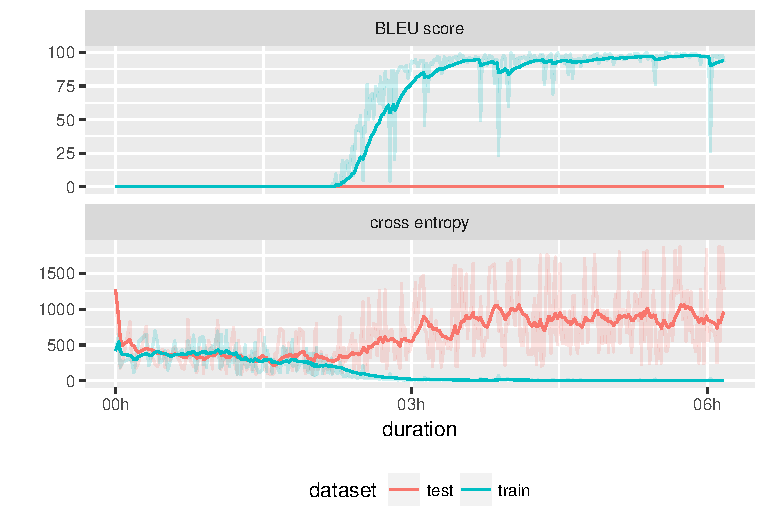
\includegraphics[scale=1]{bytenet/validation-memorize-wmt.pdf}
    \caption{Shows BLEU score and cross entropy loss for the German to English WMT NewsTest dataset. Both training and test measures are calculated on a randomly sampled mini-batch from each dataset. The exponential moving average used a forget factor of $0.1$.}
    \label{fig:result:bytenet:wmt}
\end{figure}

\begin{table}[h]
\centering
\begin{tabular}{r|p{3.3cm} p{3.3cm} p{3.3cm}}
	obs. & source & target & predict\\ \hline
  0 & Polizei von Karratha verhaftet 20-Jährigen nach schneller Motorradjagd & Karratha police arrest 20-year-old after high speed motorcycle chase & Wontin, far of the bercemal wete tower, and the Anxple pexf that deasid Therest wigh \\
  1 & Das Motorrad sowie eine Person, die der Beschreibung des Fahrers entsprach wurden später bei einem Haus im Walcott Way in Bulgarra gesehen. & The motorcycle and a person matching the description of the rider was then spotted at a house on Walcott Way in Bulgarra. & The Cotherty the fhe srone me plinethe sernid hatt col ce srmacis " forst of cotwoull, tanes ap o hirs ondithame.
\end{tabular}
\caption{Source, target and prediction on the test dataset.}
\label{table:result:bytenet:wmt-test}
\end{table}

\begin{table}[h]
\centering
\begin{tabular}{r|p{3.3cm} p{3.3cm} p{3.3cm}}
	obs. & source & target & predict\\ \hline
  0  & Zwei Anlagen so nah beieinander: Absicht oder Schildbürgerstreich? & Two sets of lights so close to one another: intentional or just a silly error? & Two sets of Gights so closento ond anotrero forentiog ther Gperbe ties wron the pllis buching thats and and ane. \\
  1 & Diese Frage hat Gutachs Bürgermeister gestern klar beantwortet. & Yesterday, Gutacht's Mayor gave a clear answer to this question. & Yesterday, Guthaltha Meyor gage in ther assuer to the ricesteon deromen to now, aing warr pepe hevern wer a sevembytich.
\end{tabular}
\caption{Source, target and prediction on the training dataset.}
\label{table:result:bytenet:wmt-train}
\end{table}

Ensuring that the optimization converges was the primary purpose of this experiment. Figure \ref{fig:result:bytenet:wmt} shows that the parameter optimization, does like in the synthetic digits problem, appear to converge just fine. Initially, there is some jitter in the cross entropy training loss, but this subsides after awhile. 

As said the test loss is not very interesting, as there is isn't enough training data to expect the model to produce meaningful results. The cross entropy on the test dataset does also show an increase after the initial decrease, which indicates some overfitting. Again, this is to be expected given the small training dataset.

More interesting is the correlation between the training cross entropy and the training BLEU score. Initially, the cross entropy decreases a lot, but the BLEU score stays at 0. It is first when the cross entropy nears 0, that the BLEU score begins to improve. This observation is quite important as it indicates that cross entropy isn't the best loss measure for the translation problem. This is because the cross entropy can be quite low if it just gets the majority of the characters almost correct, but the position must be correct. The BLEU score, on the other hand, demands that the words matches exactly, but is looser regarding the position. In particular, the cross entropy and BLEU score are not very correlated when the translation model gets a space wrong. For example in table \ref{table:result:bytenet:wmt-train} the target is ``close to'' but the prediction is ``closento''. This is very close in terms of cross entropy but is completely wrong in terms of the BLEU score, since none of the words matches. Nevertheless, the cross entropy loss is useful because its gradient in combination with softmax is easily commutable, and the BLEU score does become very high in the end, even though the correlation between cross entropy and the BLEU score is weak.

The training BLEU score is actually extremely good, it shows almost a perfect translation. Typically translation models only show a BLEU score between 15 and 25 on a test set. This is not necessarily because this the translation is wrong, but because there many different ways of translating a text correctly. The BLEU score does actually support multiple target sequences, but this rarely provided in the test dataset because of the labor demands for creating multiple translations is very high.

The only way the model can be this good is by primarily memorizing the output given the input. It is unlikely there is much understanding of the latent semantic meaning in the text. That being said, the first predictions in table \ref{table:result:bytenet:wmt-test} shows that the model understands enough grammar to use both interjection comma, and Oxford comma. It also understands that if the source doesn't end with a punctuation period then the target also should end with a period symbol. That being said, the second prediction example in table \ref{table:result:bytenet:wmt-test} also contains single quotation mark, which is not grammatically meaningful. 

Some of the above-mentioned issues could perhaps be improved by not using the target sequence in the decoder during training step. Instead, the predicted sequence could be used in the decoder input, just like in the inference model. This could solve issues like ``close to'' becoming ''closento'', as predicting space would become a more important as it indicates the start of a word. The disadvantage of doing this is that training would be slower, as the decoder can't be parallelized over the sequence. Some research suggests that one uses a hybrid model where the training loss is composed of both an assisted part and a non-assisted part, where the target sequence isn't used \cite{no-assist-train}.

Another observation is that the predicted sequences are in general a bit longer than the target sequences. This is likely because of how the sequence loss is constructed, this only measures the error where the target is explicitly known. Thus there is little penalty for predicting longer sequences than the target sequence. However, there is some penalty, because the predicted \texttt{<eos>} symbol should match the target \texttt{<eos>} symbol. This problem could be solved by padding the target sequence sufficiently with a special \texttt{<null>} symbol, and then also measure the error on part of the sequence. However, this introduces an issue where the translation model can just predict ``\texttt{<null><null><null><null>...}'' and this will in terms of cross entropy be a good match since the majority of the sequence matches. This is an easily obtainable solution for the optimizer and it can be a local minimum that is difficult to escape.

\clearpage
\subsection{WMT Translation Task}

With the ByteNet model reasonably validated in terms of generalization on the synthetic digits problem and convergence when memorizing the WMT NewsTest dataset, the ByteNet model is used on the Europarl v7 dataset for German to English translation.

\begin{figure}[h]
    \centering
    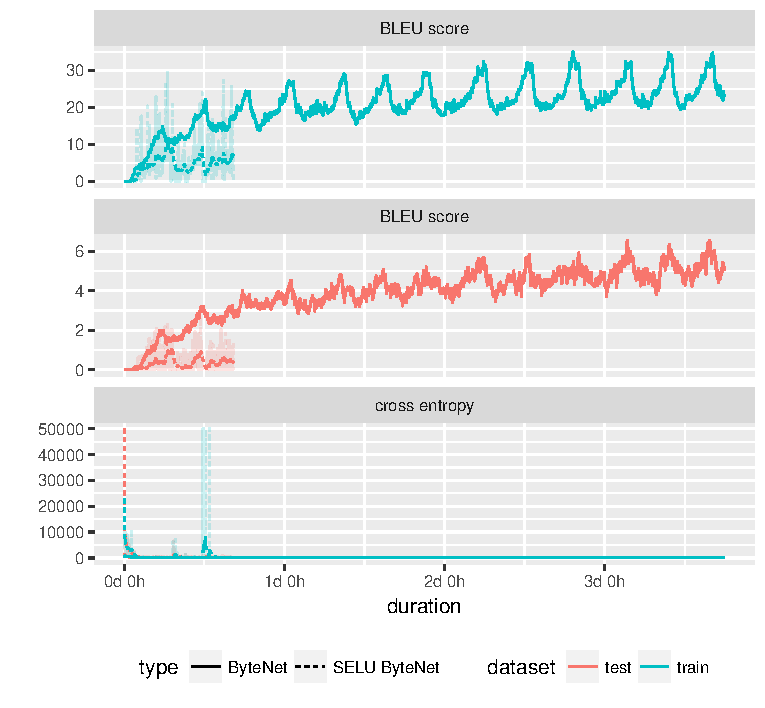
\includegraphics[scale=1]{bytenet/europarl.pdf}
    \caption{Shows BLEU score and cross entropy loss for ByteNet, trained on Europarl v7 and tested on WMT NewsTest 2015. Both training and test measures are calculated on a randomly sampled mini-batch from each dataset. The exponential smoothing used a forget factor of $0.05$.}
    \label{fig:result:bytenet:europarl}
\end{figure}

The ByteNet model has an internal dimensionality of 400, just like the model used for training on the WMT NewsTest dataset. The Adam optimizer with a learning rate of 0.0003 is used for training. This used a training mini-batch size of $4 \cdot 16 = 64$ observations and the model was trained on 4 GPUs in parallel with synchronized updates. The Europarl v7 dataset is used for training and model ran 9 epochs over the Europarl v7 dataset. The WMT NewsTest 2015 dataset is used for testing, the continues testing was done on randomly sampled mini-batches with 128 observations.

From figure \ref{fig:result:bytenet:europarl} its seen that the BLEU on the test dataset just reaches 5. This is not enough to provide reasonable meaning full translations.

\todo[inline]{Will finish section with test and training examples once the training is complete. The new results are actually somewhat encouraging and suggest a BLEU score of 15 could be reached within a week.}

\clearpage
\subsection{Performance profiling}
To understand why the ByteNet model is so slow, TensorFlow was profiled while executing the computational graph. The setup is identical to the ``Memorizing WMT NewsTest'' setup running on 4 GPUs, and the profiling was done when evaluating the 100th mini-batch.

\begin{figure}[h]
    \centering
    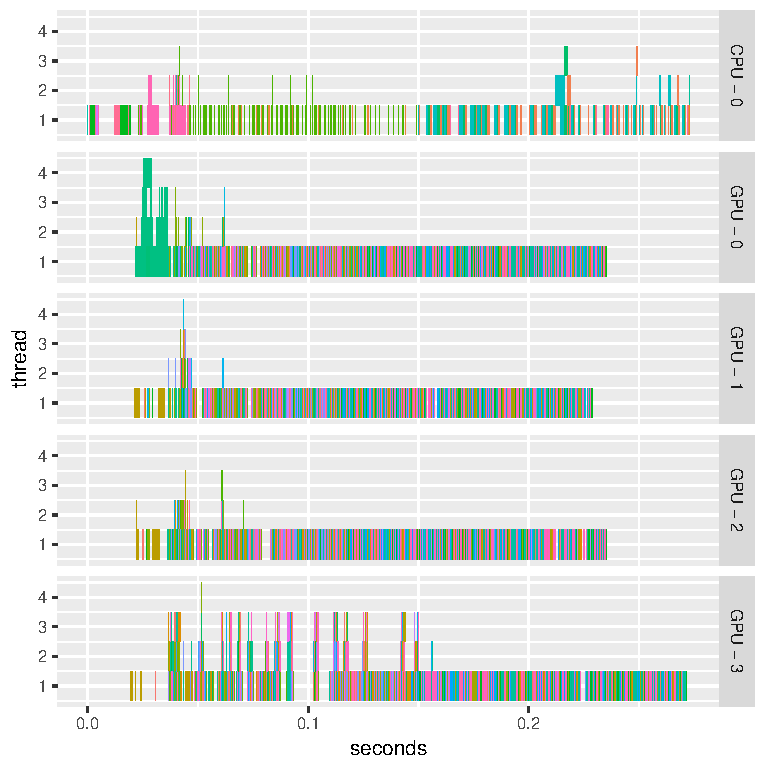
\includegraphics[width=\textwidth]{bytenet/profile-raw-gpu4.pdf}
    \caption{Shows time spend on each operation, when the operation was executed, and on what GPU/CPU it was executed. The color coding indicates the operation type, there are more than a 100 different operation types, most are specific to TensorFlow, thus the legend is not included.}
    \label{fig:result:bytenet:profile-raw}
\end{figure}

From figure \ref{fig:result:bytenet:profile-raw} it's seen that most of the time is not spend computing, but rather waiting for data to be transferred or just waiting for the TensorFlow service to queue a new computation job.

\begin{figure}[h]
    \centering
    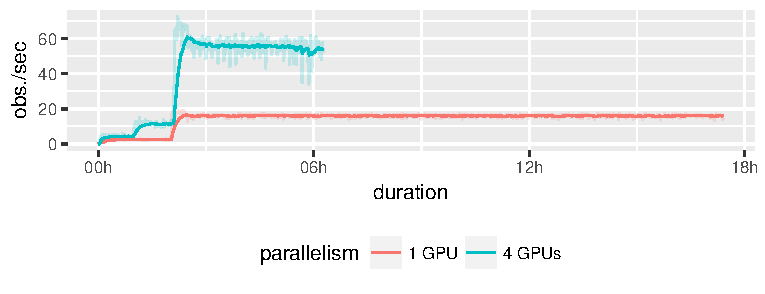
\includegraphics[scale=1]{bytenet/timing-gpus.pdf}
    \caption{Comparing observations per second, depending on the number of GPUs used.}
    \label{fig:result:bytenet:timing-gpus}
\end{figure}

By comparing the speed of how fast the ByteNet implementation processes observations depending on the number of GPUs used, one gets that about 65\% of the time is spent wait for data transference. This calculation does, in particular, make sense when comparing with 1 GPU since a 1 GPU setup will not require data transfer of any weights, as the gradients don't need to be synchronized on the CPU, but can be kept on the GPU where they are calculated.

The data transfer this does not explain all the waiting time, this can also be seen when profiling on the 1 GPU setup (appendix \ref{appendix:result:bytenet-profile}). By processing the profiling dump file, such that the waiting time is removed from the plot, one can see that about 90\% of the time not waiting for data is spend waiting for the TensorFlow service to queue computations. This is seen in figure \ref{fig:result:bytenet:profile-raw} and appendix \ref{appendix:result:bytenet-profile}.

\begin{figure}[h]
    \centering
    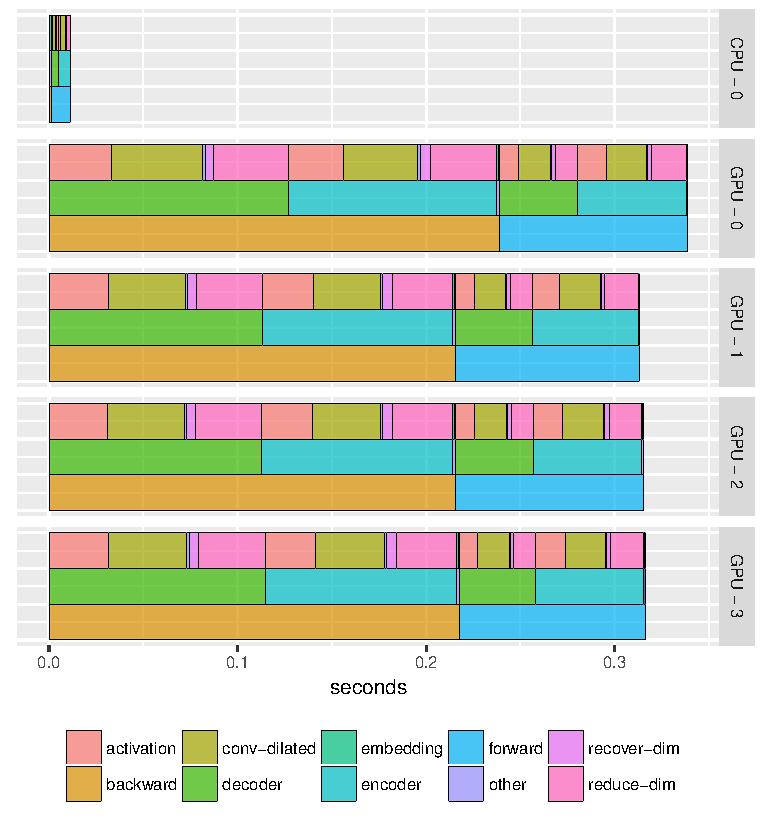
\includegraphics[scale=1]{bytenet/profile-grouped-gpu4.pdf}
    \caption{Shows time spend executing operations in each part of the ByteNet model, this excludes the waiting time. Each part exists in a hierarchy, which is visualized as levels. The bottom level is the least detailed level, it just splits the model in the backward and forward pass. The next level, splits the model in the encoder and decoder. The last level at the top, primarily splits the ByteNet Residual Blocks.}
    \label{fig:result:bytenet:profile-raw}
\end{figure}

It is likely that the data transfer part could be optimized, but in general, this isn't easy and there are practical limitations to how much it can be improved. It is much more likely that the waiting time regarding the TensorFlow service could be improved.

TensorFlow works with a computational graph. Each atomic operation, like an element-wise addition or a matrix multiplication, is a node in this graph and the edges describe the dependencies. The TensorFlow service will watch the graph and execute any node (atomic operation) where all the dependencies are satisfied, it will even execute multiple nodes in parallel if possible. This process repeats until all nodes have been computed and the end result is obtained.

This computational graph is a good strategy, but the current TensorFlow implementation of it is very naive. TensorFlow uses no-op and identity operations, which only exists because of TensorFlow semantics, but don't need to be executed. However, in the current state of TensorFlow, it just executes all nodes naively. There are also numerous of atomic operations that could be fused into one atomic operation. An example is batch normalization that involves quite a few element-wise operations, all these are executed separately but could be combined into a single atomic operator. All these atomic operators are what cases the waiting time, the TensorFlow service needs to walk the computational graph and more importantly just launching GPU kernels also introduces wasted time.

The TensorFlow team is aware of the current limitations and are in the process of solving these issues, but using a Just In Time compiler that can automatically fuse many of these operations, but so fare this is in an experimental state and performs very poorly when running on multiple GPUs \cite{citation-needed}.
